\documentclass[10pt,twocolumn,letterpaper]{article}

\usepackage{cvpr}
\usepackage{times}
\usepackage{epsfig}
\usepackage{graphicx}
\usepackage{amsmath}
\usepackage{amssymb}
\usepackage{url}
\usepackage{algorithm}% http://ctan.org/pkg/algorithms
\usepackage[noend]{algpseudocode}% http://ctan.org/pkg/algorithmicx
\usepackage{subcaption}

% Include other packages here, before hyperref.

% If you comment hyperref and then uncomment it, you should delete
% egpaper.aux before re-running latex.  (Or just hit 'q' on the first latex
% run, let it finish, and you should be clear).
\usepackage[breaklinks=true,bookmarks=false,draft]{hyperref}

\cvprfinalcopy % *** Uncomment this line for the final submission

\def\cvprPaperID{****} % *** Enter the CVPR Paper ID here
\def\httilde{\mbox{\tt\raisebox{-.5ex}{\symbol{126}}}}

% Pages are numbered in submission mode, and unnumbered in camera-ready
%\ifcvprfinal\pagestyle{empty}\fi
\setcounter{page}{1}
\begin{document}

%%%%%%%%% TITLE
\title{Mathematical Expression Recognizer}

\author{ChanMin Kim
\thanks{
    Author names are listed in alphabetical order. We've contributed to the project equally.
}
\qquad HeeHoon Kim \qquad Sanghyeok Park\\
Department of Computer Science and Engineering\\
Seoul National University\\
{\tt\small kcm1700@snu.ac.kr, csehydrogen@gmail.com, pps987@snu.ac.kr}
% For a paper whose authors are all at the same institution,
% omit the following lines up until the closing ``}''.
% Additional authors and addresses can be added with ``\and'',
% just like the second author.
% To save space, use either the email address or home page, not both
}

\maketitle
%\thispagestyle{empty}

%%%%%%%%% ABSTRACT
\begin{abstract}
    We implemented simple mathematical expression recognizer using Convolutional Neural Network (CNN).
    Our recognizer takes pictures of one line math expression, and generates TeX form of the expression.
    It can only recognize digits, some arithmetic operators, parenthesis, $\pi$, and $e$.
    Our CNN model is modified LeNet, and the network was trained and tested with Caffe, using MNIST and CROHME.
    MNIST is a data set of handwritten digits, which contains 60000 train and 10000 test images.
    CROHME is a data set of handwritten digits and other symbols that we need. It has 38248 images.
    With those data sets, our model shows about 98\% accuracy on test set.
    Our recognizer works with following steps; normalization, segmentation, and recognition.
    In normalization part, we used local thresholding method.
    In segmentation part, we applied Flood-Fill and our own merging algorithm.
    Finally, in recognition part, we obtain the probability for each symbols with our own network;
    however, we used dynamic programming approach to avoid nonsense expressions.
    In order to determine which expression flow makes sense,
    we defined states contains probabilities with respect to a writen component, a parenthesis depth, and a kind of guessed symbol. % hmm...
    We calculated all states in $O(n^2 \sigma^2)$ time using dynamic programming, which is enough fast.
    To take the maximum probability of states, we can avoid nonsense expressions, such as $1(+30$.
    This approach was very important.
    By our confusion matrix of our model, there exist miss rates over than 10\%.
    However, if symbols that make confusion are similar but in different kind, we can handle with dynamic programming.
    We used another information of expression: the context of expressions; therefore, we could get better results.
    We made a web demo application using above approachs at \url{http://chanmin.kim/image-expr/}.
\end{abstract}

%%%%%%%%% BODY TEXT
\section{Introduction}

We implemented a simple mathematical expression recognizer which takes pictures of
math expressions and generates TeX form of expressions. Our program has some restrictions.
It can only recognize expressions that has only digits, arithmetic operators($+, -, \times, /, \div$),
parentheses, $\pi$, $e$. Expressions also should be in one line, and not have
superscripts or subscripts. Background should be bright, and the expression should be dark.

We devided this problem into three parts, normalization, segmentation, and recognition.
In normalization part, we binarized our gray scale natural image, and rotated it to
fit in straight rectangle box. In binarization, we applied local thresholding method.
Then we use ternary search method to find best angle we have to rotate.

In segmentation part, basically we splited binarized symbols into connected components
using Flood-Fill. However, we had to merge components into same symbol. For example,
$=$ symbol is one symbol but it has two components. Because our expressions is in only
one line, we measured only X-coordinates and overlap ratio of components. If one of the
two components overlap ratio is larger than the threshold, we merged those components
into same symbol. We chose the threshold $50\%$.

In recognition part, we determined which symbol each merged component actually is.
The probability for each component to be a specific symbol was calculated from neural network.
Our neural network model is modified LeNet\cite{LeNet}.
The network was trained and tested with Caffe, using MNIST\cite{MNIST} and CROHME\cite{CROHME} data sets.
In order to prevent nonsense predictions (consecutive operators, unmatched parentheses, etc.), we used dynamic programming approach.

% TODO
% result & this research's contribution (accomplishment) to this field

\section{Background}

There are a number of prior studies in the field of recognition of mathematical expressions.

Michael Nielsen\cite{MichaelNielsen} wrote an introductory book on neural networks.
The book describes the basics of neural network.

MNIST\cite{MNIST} data sets are famous for handwritten digits.

One of the most popular mathematical expression recognition competition is CROHME,
which stands for
`Competition on Recognition of Online Handwritten Mathematical Expressions'\cite{CROHME}.
They provide rich train data set and test data set of handwritten mathematical expressions
in InkML. InkML is a file format for representing trace of handwriting.


There was a student project by Vitali Sepetnitsky and Yakir Dahan\cite{OCRMATH}, which recognizes book printed mathematical formulas.
There was also a related course project by Alistair Dobke and Mark Mann\cite{OCRMATH2}. The project recognizes handwritten mathematical expressions just as our project.



\section{Approach}

% TODO:
% 우리들의 문제 해결은 어떻게 했는지 쓰기. 여기를 심혈을 기울여 쓰는 게 맞을듯
%
% 생각하고 있는 구조.
%
% - 알고리즘 (중요)
%  - neural net training
%    - training/test 데이터 가공 (Done)
%    - 사용한 파라미터와 구조 설명(conv1,conv2,conv3,ReLU,inner product, dropout, output layer(softmax) 언급 다 필요. conv는 kernel size 및 개수 표현) (Done)
%  - normalization
%    - binarization: local threshold method 알고리즘 구체적으로 설명. 이미지 또는 pseudo code 필요
%    - rotation: 수식으로 설명. ternary search는 언급하면 될듯
%  - segmentation
%    - flood fill
%    - merging intervals 알고리즘 설명 및 PPT 이미지 활용
%    - dot recognition: 최대 높이/ 최저 높이 추정하고 그것을 기준으로 점 여부 판별하고 위치에 따라 .과 \cdot 분리
%  - dynamic programming
%    - 불가능한 수식 거르는 규칙
%      - 괄호
%      - opening parenthesis '(' 직후 binary 연산자(unary는 허용) 확률 0
%      - closing parenthesis ')' 직후 binary 연산자(unary는 허용) 확률 0
%      - 등 다양한 규칙 썼는데, 이걸 서술할 것.
%    - softmax 결과를 이용한 확률 곱 최대화.
%    - DP state 정의 및 의미
%    - 기대되는 효과: 실제 digit 단위 실험 결과를 보면 confusion matrix에서 /,(,),1 등이 자주 헷갈리고 3,{가 헷갈리고, 9,}가 헷갈리는데 이러한 경우 어느 게 맞는지 효과적으로 추론.
% - 프로그래밍 언어: python
% - 사용한 내용: caffe(뉴럴넷), Pillow(이미지 처리용), numpy(각종 계산용), scipy(마찬가지), django(웹데모개발용)
%
%
%
%

% TODO: 여기다가 Approach section의 구조 설명을 추가한다.

\subsection{Preprocess}

Since we use neural network, preprocesses, like data generation, modelling, and training, are as important as our main algorithm.
We covered details in this section.

\subsubsection{Training and Test Data Generation}

Widely used databases of handwritten mathematical symbols have different formats.
We needed to convert them in a uniform format which is easy to train and test under Caffe framework.
We used MNIST and CROHME, which were enough for our purpose.

MNIST data are available as idx files, which contain 60000 train images and 10000 test images.
Each image is a anti-aliased grayscale handwritten digit image, which is normalized to 20 by 20 image preserving aspect ratio, and centered in 28 by 28 image by computing the center of mass of pixels.
We used this format as standard for training.

CROHME data was used to cover symbols other than digits.
We only used data containing digits, basic operators(+, -, $\times$, $\div$, /, =), parentheses([, ], (, ), \{, \}), $\pi$, and e.
They are formatted as inkml, which contains stroke information only.
Lines are generated by linear interpolation from coordinates.
Then we applied anti-aliasing with 4 strengths since stroke width is undefined.
Finally, we converted them into the same padded-size image as MNIST.

From two databases we get 212992($=60000+38248*4$) train images and 21772($=10000+2943*4$) test images.
We merged them into LMDB database file for faster input.

\subsubsection{Neural Network Modeling}

\begin{figure}[t]
\centering
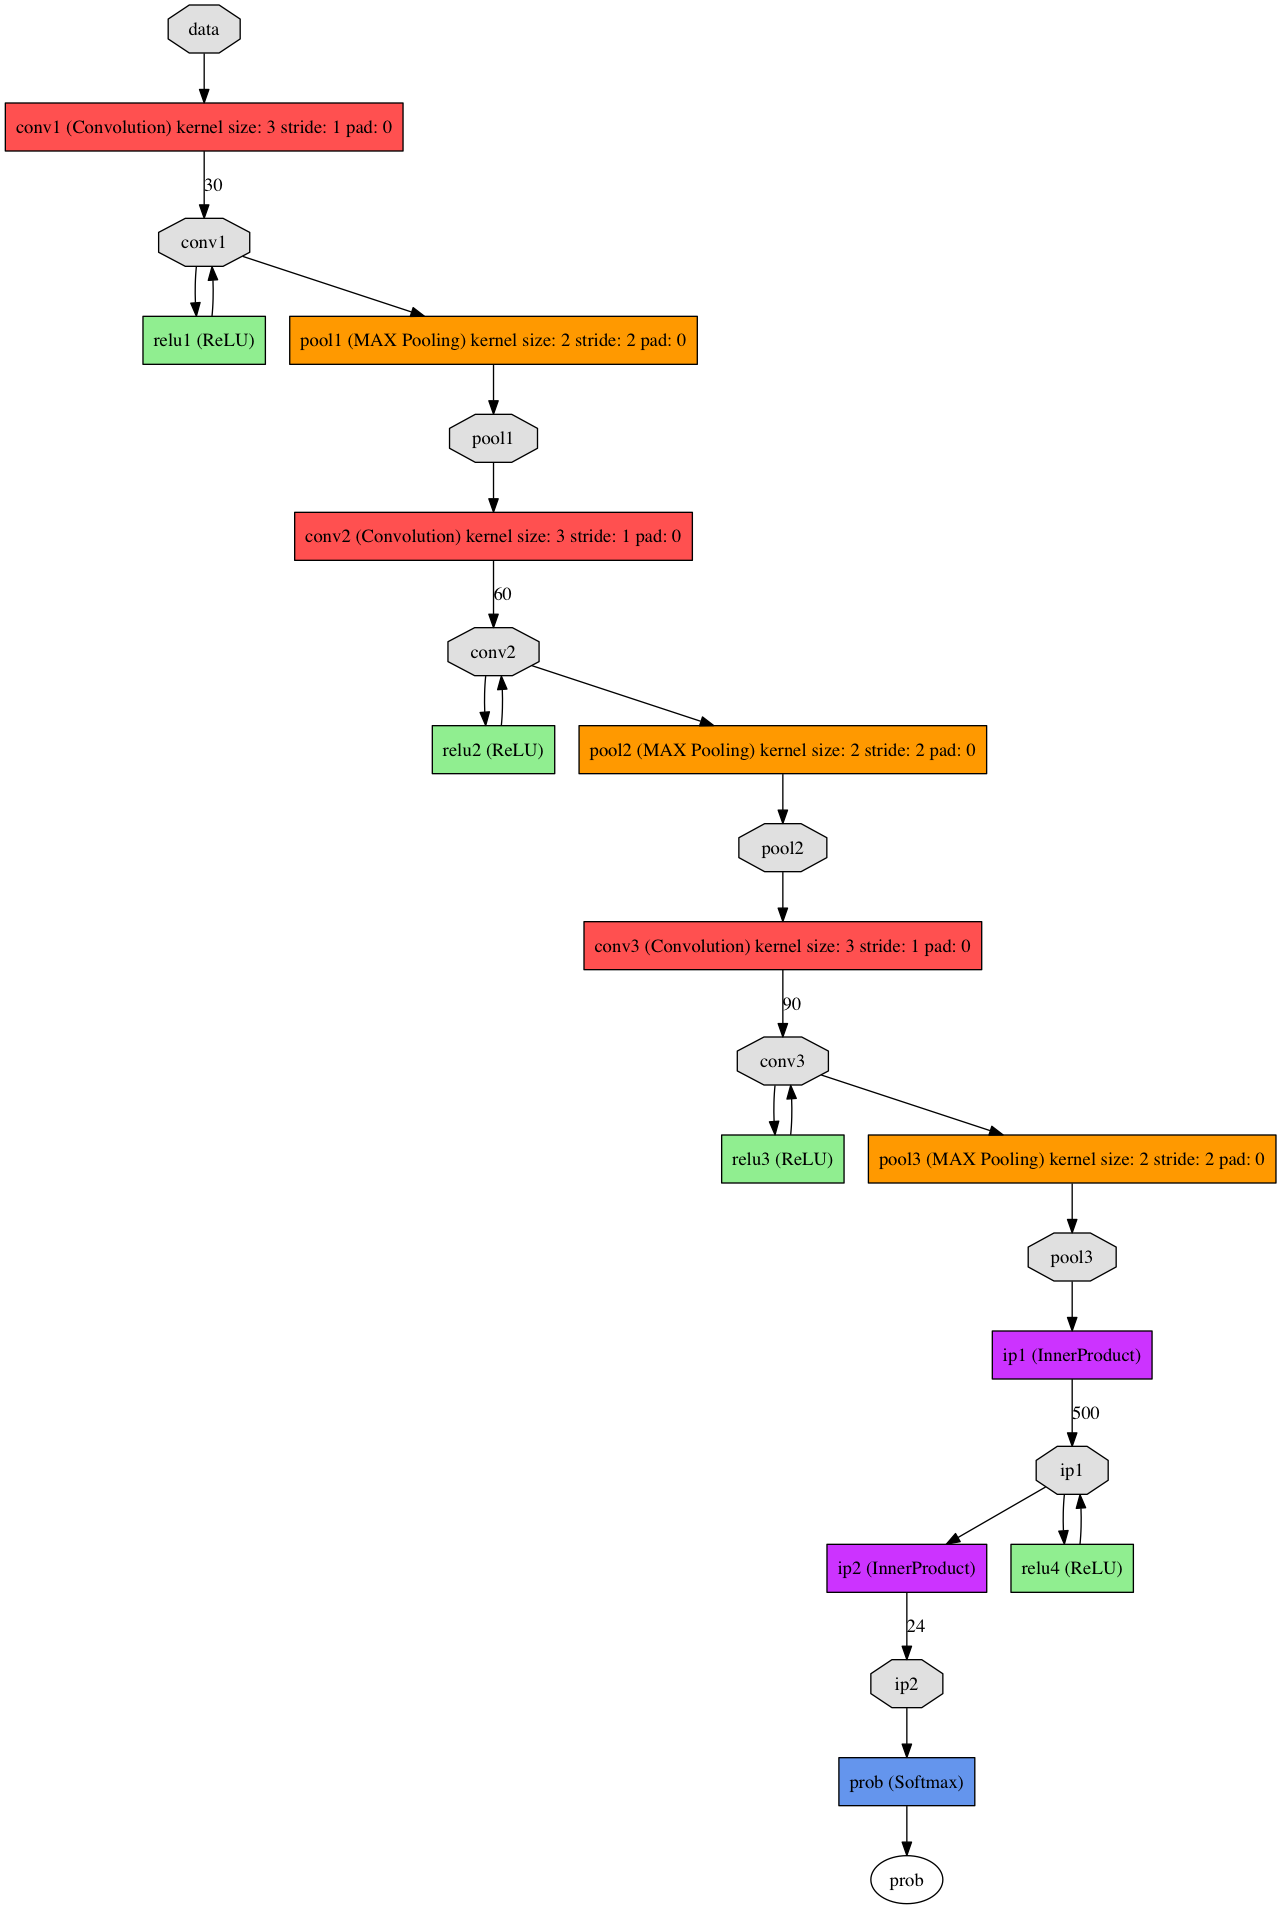
\includegraphics[width=0.9\linewidth]{img/model.png}
\caption{Our neural network model}
\label{fig:model}
\end{figure}

Our network model should be proper to categorize handwriting symbols.
We took approach to take existing model, LeNet, and modify for better predictions.
Our full model is depicted in Figure \ref{fig:model}.

First part of the model consists of 3 convolution steps, compared to 2 in LeNet.
Each step has Convolution layer, ReLU layer, and Pooling layer.
They output 30, 60, 90 channel images of decreasing size, respectively, which are also larger than LeNet.

Convolution layer picks up overall features of images from previous layers.
LeNet uses kernel of size 5, but we reduced them to 3.
Since we try to categorize twice more symbols from the same size images, large kernel has danger of losing too much information. 

ReLU layers are added for better prediction.
We used leaky ones, i.e., negative slopes are $0.01$.
It is known that ReLU layers increase non-linearity, resulting in better and faster train.
Dropout with probability $0.5$ is also applied to prevent overfitting and make train faster.

Pooling layers are also placed after ReLU layers.
They use max function to decrease variance during detection.
Also, kernel of size 2 and stride of 2 effectively decrease image size to half in each dimension.

Latter part of the model consists of 2 InnerProduct layers and a Softmax layer.
InnerProduct layers are fully-connected layers, which don't have spatiality anymore and prepare for output.
Second InnerProduct layer produces 24 dimension vector, which is the same with the number of kinds of symbols.
Then Softmax layer takes this vector and outputs estimated probabilities for each symbol.

\subsection{Algorithm}

Our algorithm consists of several steps. We first binarize the image and rotate the image.
Then we segment the image into characters.
The final step is to apply dynamic programming to guess each symbols.

\subsubsection{Binarization}

\begin{algorithm}
\caption{Binarization} \label{binarization}
\begin{algorithmic}[1]
\Function{binarize}{}
\State \texttt{image} $\gets$ grayscale(\texttt{image})
\State \texttt{ns} $\gets$ \textbf{max} (\texttt{width} / $W_{large}$, \texttt{height} / $W_{large}$)
\State \texttt{nearsum} $\gets$ \texttt{image} $\ast$ (\texttt{ns} $\times$ \texttt{ns} mean filter) \\
\Comment{$\ast$: convolution operator}
\State \texttt{fs} $\gets$ \textbf{max} (\texttt{width} / $W_{small}$, \texttt{height} / $W_{small}$)
\State \texttt{farsum} $\gets$ \texttt{image} $\ast$ (\texttt{fs} $\times$ \texttt{fs} mean filter)
\State \texttt{threshold} $\gets \frac{1}{6}$ \textbf{min} (\texttt{nearsum} - \texttt{farsum})
\State \Return \texttt{nearsum} $<$ \texttt{farsum} + \texttt{threshold}
\EndFunction
\end{algorithmic}
\end{algorithm}

The binarization algorithm consists of several steps as shown in \textbf{Algorithm \ref{binarization}}.
The algorithm caculates nearby pixel average and wider area average for each pixel.
Then the function calculates the differences and check the difference against the \texttt{threshold}.
The result is \texttt{height} $\times$ \texttt{width} binarized image.
$W_{large}$ and $W_{small}$ are parameters to the algorithm.
We used 350 and 30 for $W_{large}$ and $W_{small}$ respectively.

\begin{figure}[t]
\begin{center}
   \subcaptionbox{global thresholding}{
        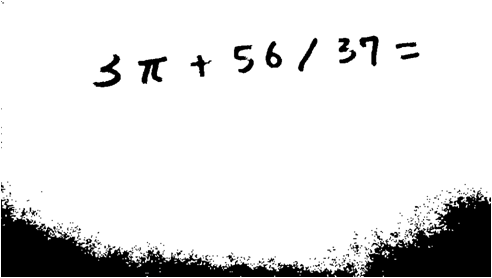
\includegraphics[width=0.47\linewidth]{img/global.png}
   }
   \subcaptionbox{local thresholding and rotation}{
       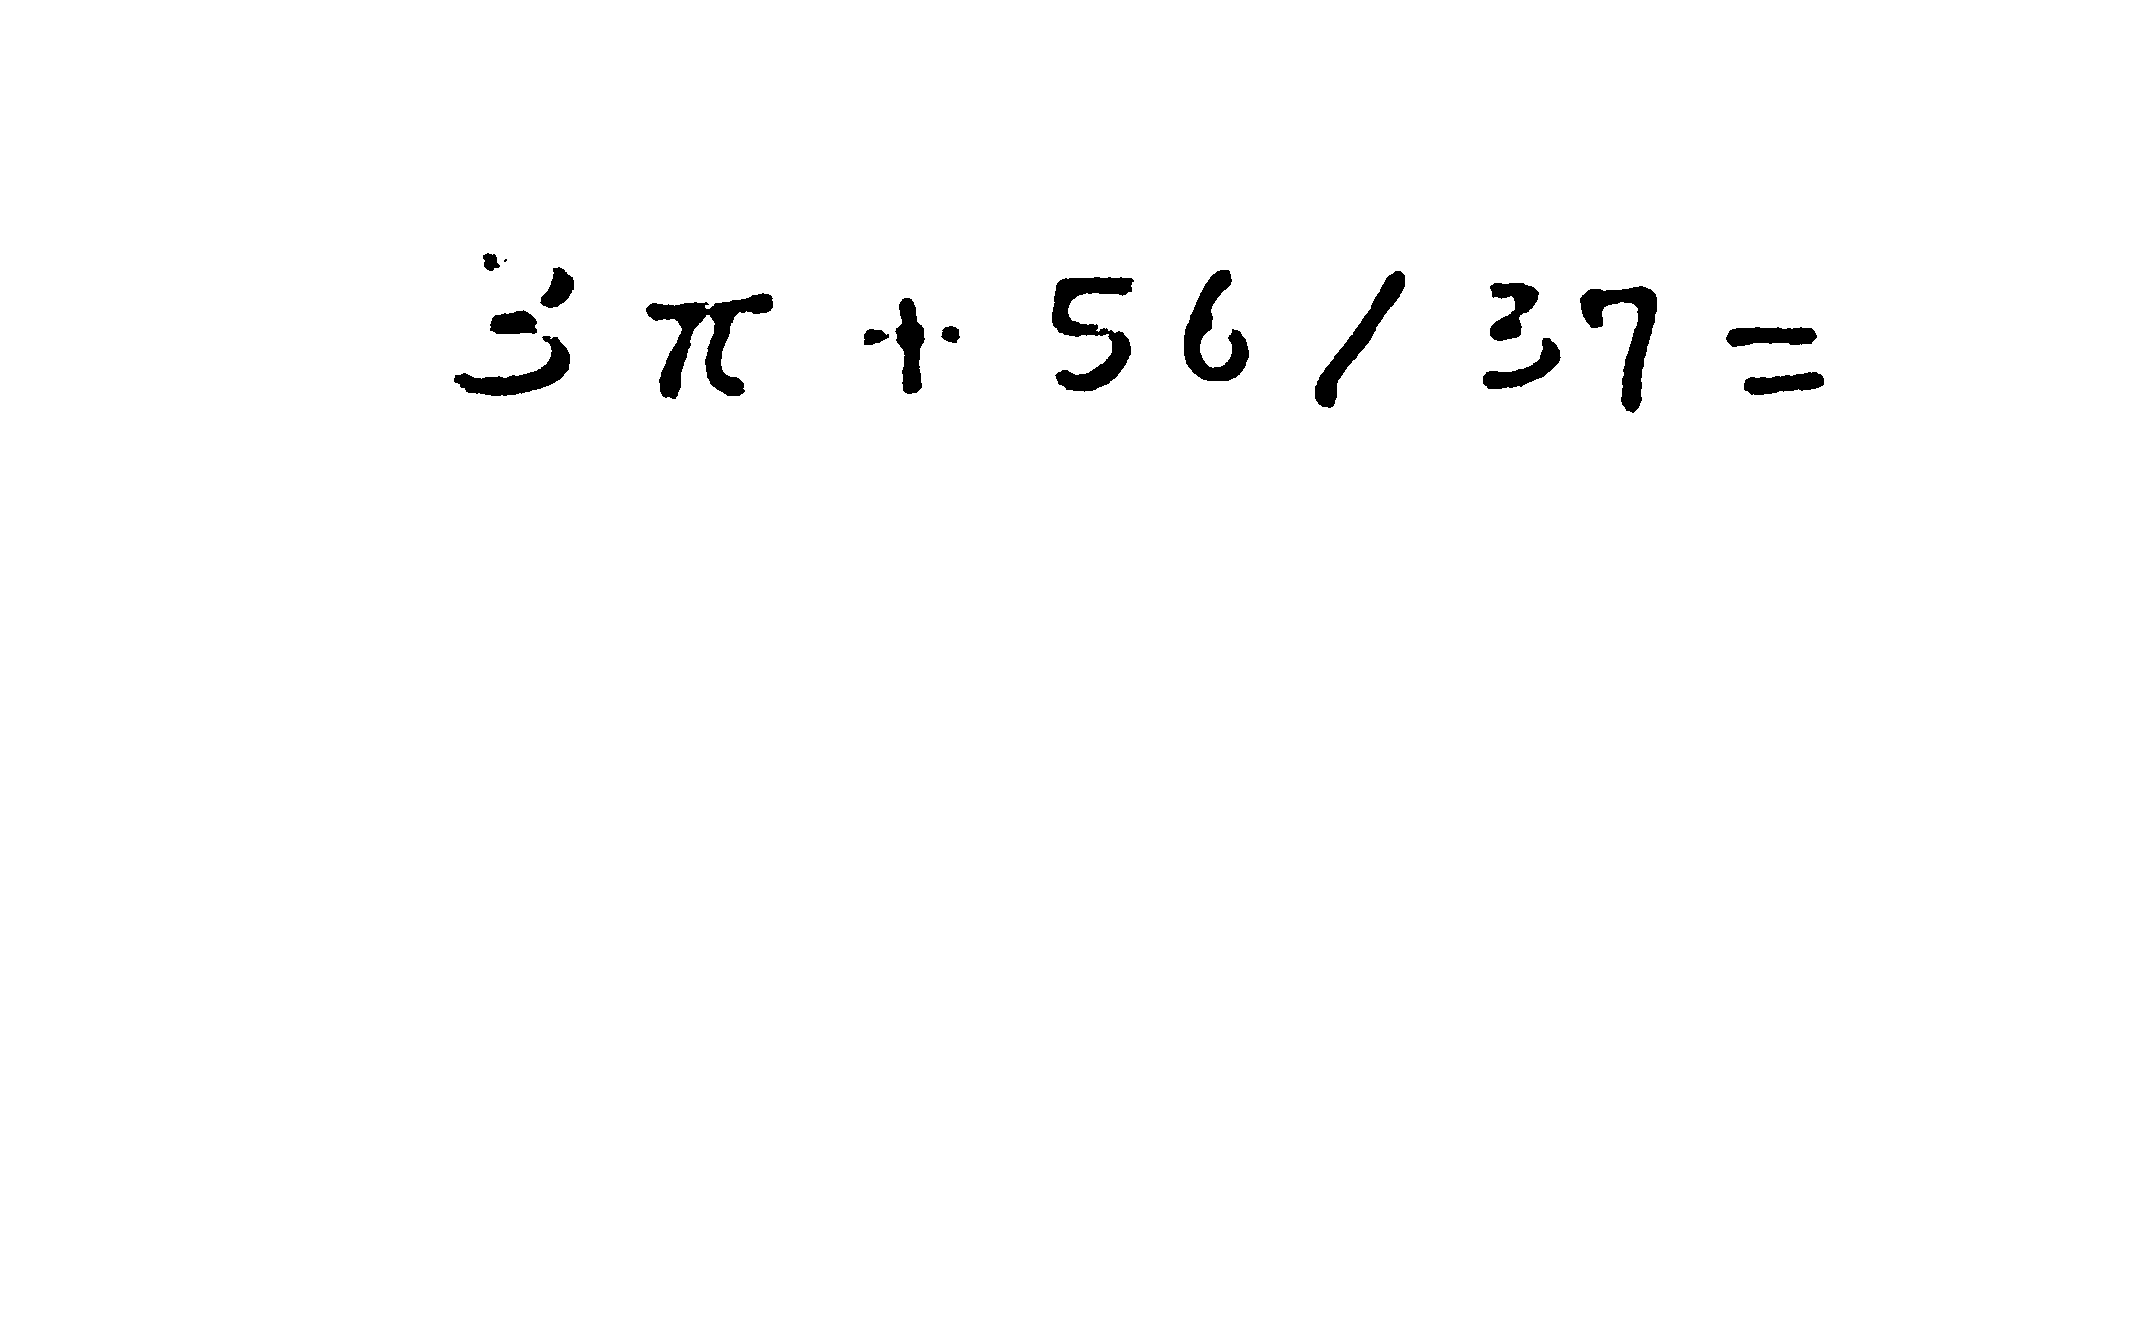
\includegraphics[width=0.47\linewidth]{img/local.png}
   }
\end{center}
   \caption{It is nearly impossible to separate the text by usual thresholding methods. }
\label{fig:thresholding}
\end{figure}

Our binarization method uses only neighborhood information.
We were forced to apply local thresholding method instead of global thresholding method.
Some parts of the background were sometimes darker than the text.
See Figure~\ref{fig:thresholding} for example.

\begin{figure}[h]
\begin{center}
   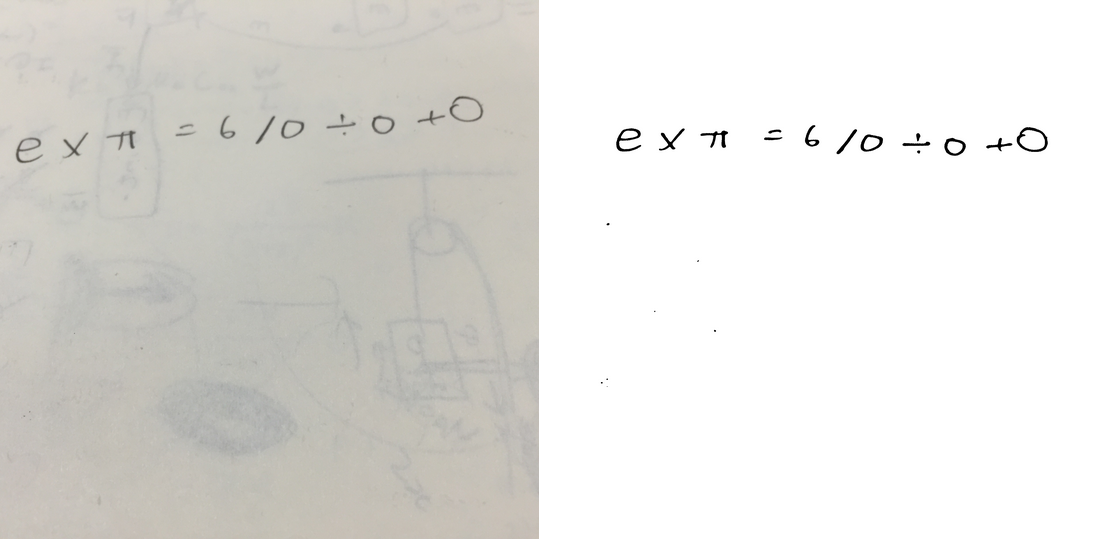
\includegraphics[width=0.97\linewidth]{img/noisybg.png}
\end{center}
\caption{Example image of noisy background}
\label{fig:noisy}
\end{figure}

\subsubsection{Rotation}

We rotated the image by appropriate angle for better segmentation and recognition.
We set the object function $D$:
\begin{equation}
\label{eq:rotation-objective}
D(\theta) = \textrm{std}[x_i \sin{\theta} - y_i \cos{\theta}] \textrm{ for all black pixels } i
\end{equation}
This function means the standard deviation of $y$ coordinates of the rotated image.
We want to minimize the object function $D$ with regarding to $\theta$.

Our algorithm finds the best angle by using ternary search on range $[-\frac{\pi}{6}, \frac{\pi}{6}]$.
Since finding the best angle is straight-forward, we'll skip the details.
See Figure~\ref{fig:thresholding} and Figure~\ref{fig:noisy} to see the effect of the rotation step.



\subsubsection{Flood Fill}

Basically we assume that connected pixels are in same symbol. Therefore, using Flood-fill,
we decomposed image into components which contain only connected points.
However, it is not enough to determine symbols.

\subsubsection{Region Merge}

There exist two problems using only Flood-fill.

First, some symbols have several disconnected components. For example, $\div$ % 나눗셈 기호?
has at least three disconnected components.
Second, noise problem; some connected components in ideal might be written
by several disconnected components.

To solve those problems, we should merge some components. One of the simple method of merging
is assuming components are in same symbol if and only if there exist points of each components
which have same X-coordinates. However, this simple method makes another problem.

\begin{figure}[t]
    \begin{center}
        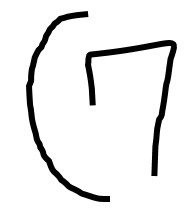
\includegraphics[width=0.1\linewidth]{img/little_overlapping.png}
    \end{center}
    \caption{'$($' and '$7$' shares few X-coordinates}
    \label{fig:little_overlapping}
\end{figure}

In Figure \ref{fig:little_overlapping}, '$($' and '$7$' component shares few X-coordinates;
therefore, they will be merged.
However, we expect that those components should not be merged.

Therefore, we should restrict our merging method. Our idea is that merge two components
if and only if one of the components has common X-coordinate interval more than $50\%$.
In formal, let $A$ and $B$ be two components which we want to determine whether we should merge.
Let $A_l$, $B_l$ be leftmost point of $A$ and $B$, also $A_r$, $B_r$ be rightmost point of $A$ and $B$, respectively.
Let $[c_l, c_r]$ be interval that is $[A_l.x, A_r.x] \cap [B_l.x, B_r.x]$ if it exists.
Finally, let $d$ be $c_r - c_l$.
Then, we merge $A$ and $B$ if and only if
\begin{subequations}
\label{eq:mergecondition}
\begin{align}
    \frac{d}{A_r.x - A_l.x} &> 0.5 \ \text{or} \\
    \frac{d}{B_r.x - B_l.x} &> 0.5
\end{align}
\end{subequations}

If we sort components with decreasing order of leftmost point of each component,
we can easily apply merging algorithm in linear time.

\begin{figure}[t]
    \begin{center}
        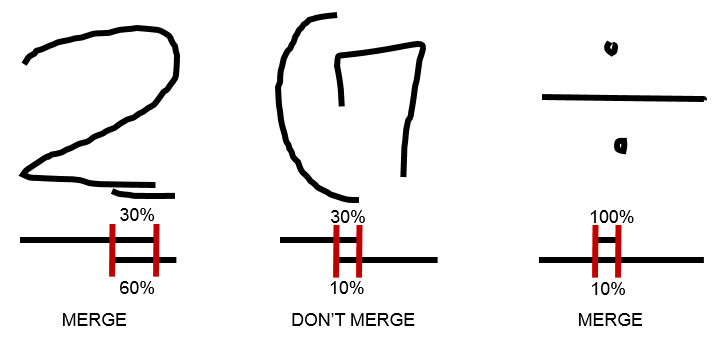
\includegraphics[width=0.8\linewidth]{img/merging.png}
    \end{center}
    \caption{Examples of merging algorithm}
    \label{fig:merging}
\end{figure}

See Figure \ref{fig:merging} to obtain that how this algorithm works and solves problems.

\subsubsection{Single Symbol Recognition}

Now we know which symbol each black pixel belongs to.
To use our trained neural network, we should transform each symbol into standard input image form, as mentioned in train data generation.
For $i$-th symbol, we extracted minimal area that contains all black pixels of the $i$-th symbol.
Then the area was resized into 20 by 20 image with anti-aliasing technique, and 4 pixel padding was added to each side.

We processed the image with our neural network, and we get $P_i$, 24-dimension vector for the $i$-th symbol.
The dimension is determined by the number of symbols that we selected.
See Table~\ref{tbl:symbollist} for full list of symbols.

The output layer of our neural network model uses softmax function.
Therefore, we can interpret $j$-th value of the vector, $P_{i,j}$, as the predicted probability of the $i$-th symbol being $j$-th class.
Taking $argmax$ on $j$ gives us the most probable class for the $i$-th symbol.

However, probability itself is not enough for parsing whole expression, since we don't benefit from context analysis.
Thus, our algorithm goes for another step, Dynamic Programming, with probabilities as some initial values.

\subsubsection{Dynamic Programming}

We finally guess the symbols in this stage.
It might be okay to just guess the segmented symbols independently,
but we did more to get better result.

We have put some restrictions on guessing.
We know that parentheses of correct mathematical expressions are matched correctly.
For example, $(1 + 4($ doesn't make sense.
We also know that duplicate operators doesn't appear in expressions except for
unary operators. For example, $3 \times \div 4$ doesn't make sense.
There are more restrictions that can be used for guessing.

Here are some of the rules that is used in our algorithm.
\begin{itemize}
\item Parentheses are correctly matched.
\item There are no digits right after $\pi$ and $e$.
\item There are no duplicated binary operators.
\item There are no binary operator after opening parentheses.
\item There are no operator before closing parentheses.
\item $\cdots$
\end{itemize}

We made a dynamic programming algorithm to make use of the rules above.
Let's define a function $d(i, open, kind)$ for DP.

$d(i, open, kind) := $ Maximum probability of the guess
when the first $i$ segmented parts are used, the parenthesis is opened $open$ times, and
the last character was guessed as $kind$-th symbol.

Then the formula \ref{eqn:dprec} for calculating function $d(i, open, kind)$ look like below.

\begin{equation}
\label{eqn:dprec}
d(i, open, kind) = \max
\begin{cases}
1 \text{\quad if $(i,open,kind) = (0,0,\Box)$ } \\
0 \text{\quad if $i$, $open$, or $kind$ is invalid} \\
0 \text{\quad if restricted by some rules} \\
P_{i,kind} \cdot d(i-1, open-1, ?) \\
\text{\quad if $kind$ is $(, \{, [$ } \\
P_{i,kind} \cdot d(i-1, open+1, ?) \\
\text{\quad if $kind$ is $), \}, ]$ } \\
P_{i,kind} \cdot d(i-1, open, ?) \\
\end{cases}
\end{equation}

Note that the above recurrence formula is just for a brief description.
There are some more cases to consider to implement.

We also have to record what states were used to find out exactly what symbols were guessed.
For example, one might want to define the following function.
$b(i, open, kind) := $ Previous $d$ state that is used to make $d(i, open, kind)$
as large as possible.

Not every segmented part is a symbol. Some of the segmented parts could be a noise in the picture.
So we have added the probability of whitespace symbol.
We have defined the probability of whitespace symbol so that every black pixel decreases the chance exponentially.

Dot symbols are not trained in our neural network model.
We have picked two dot symbols, `.' and `$\cdot$',
namely decimal point and multiplication dot.
We first guessed the bottom line and the top line of the expression.
The lines were picked so that 95\% of the black pixels are above/below the line.
Let's say the height is the distance between the bottom line and the top line.
If width and height of the segmented parts are smaller than $\frac{1}{6}$ of the height,
we consider this part as a dot.
Deciding whether the dot is a decimal point or a multiplication dot depends on the $y$ position of the segmented part.
Internal divison of the height in 1:3 ratio worked fine.

The time complexity of the Dynamic Programming step is $O(n^2 \sigma^2)$ where $n$ means the number of segmented part and
$\sigma$ means the number of symbols used. Therefore this step is reasonably fast.


\subsubsection{Combining the steps}


Finally our algorithm looks like the following \textbf{Algorithm  \ref{combined}}
\begin{algorithm}
\caption{The whole algorithm}
\label{combined}
\begin{algorithmic}[1]
\State \texttt{Image} $\gets$ \texttt{BINARIZE(Image)}
\State $\theta_{best}$ = Find the best $\theta$ of $D$.
\State \texttt{Image} $\gets$ \texttt{Rotate(Image, $\theta_{best}$)}
\State \texttt{Sections} $\gets$ \texttt{FloodFill(Image)}
\State Sort \texttt{Sections} by the start $x$ coordinate.
\ForAll {\texttt{A} $\in$ \texttt{Sections}}
    \State \texttt{B} $\gets$ the next element of \texttt{A}
    \If {formula (\ref{eq:mergecondition}) is satisfied}
        \State Remove \texttt{A} and \texttt{B} from \texttt{Sections}
        \State $[c_{l}, c_{r}]$ $\gets$ Merge \texttt{A} and \texttt{B}
        \State Add $[c_{l}, c_{r}]$
    \EndIf
\EndFor
\ForAll {\texttt{S} $\in$ \texttt{Sections}}
    \State Calculate $P$ by convolutional neural network.
\EndFor
\State Calculate $d(i, open, kind)$ and $b(i, open, kind)$
\State Backtrace the calculations to reveal the guess.
\end{algorithmic}
\end{algorithm}


\subsection{Environments}

We used Python 2.7 as our main programming language.
We used caffe and its python binding for neural network.
We used Pillow for basic image manipulation and numpy \& scipy for faster calculation.
We used Django web framework for the web demo.

\section{Experiments}

%
% 여기다 적을 거
%
% 1. symbol recognition 결과
% 테스트 데이터 생성 방법:
%   Dataset: CROHME 것을 사용한다. inkml 파일에서 우리가 대상으로 하는 symbol만 추린다. 굵기 별로 생성한다. 학습에 CROHME의 training set 사용. 평가에 CROHME의 test set 사용함.
%   softmax로 나온 결과 layer에서 argmax가 실제랑 같은지 비교
% 결과:
%   Neural Network 학습 결과 filter visualize
%   Neural Network 학습 결과 실제 샘플 convolution 결과 테이블.
%   confusion matrix. 그리고 confusion matrix의 자주 틀리는 부분들 이유 간략히 서술.
%   전체 정확도 및 신뢰 구간 구하기.
%
% 2. 실제 이미지 입력 (모두 web demo에서 참고하기) 이건 qualitative밖에 얘기 못할듯. 주목할만한 오류들 적기.
%   방법: 수식을 제시하고 해당 수식을 몇 명에게 handwriting을 받아서 수행
%
% 3. 전체 식이 우리 인식 가능한 symbol로만 이뤄진 경우 테스트?
%

\subsection{Single Symbol Recognition}

Before we run into our algorithm, neural network prediction accuracy should be tested.
As mentioned in preprocess section, we used one-symbol images generated from CROHME as train and test data.
Caffe framework was used in neural network training, which automates forward pass, compare output with ground truth, and tuning internal variables with backpropagation.
For efficient training, mini-batch of 64 images were passed at the same time in each step.
Learning rate decreased inversely starting from $0.001$, and iterations are done 10000 times.

Trained model shows about 98\% accuracy on test set.
From confusion matrix(Figure \ref{fig:confusion_matrix}), we can find out which symbol our neural network didn't predict well.
Here are noticeable cases:
\begin{itemize}
\item Symbols similar to a vertical line

/, 1, $[$, $]$, $\{$, and $\}$ fall into this case.
Although some of them even show $>10\%$ error rates, this is not a big problem.
Since / is operator, 1 is number, and others are parentheses, dynamic programming can remove improbable cases with context.
Among parentheses, we can reduce erroneous prediction by handling all parentheses as ( and ), \ie, only one set of opening and closing parentheses.

\item Similar symbols, but in different kind

7 with + and =, $\pi$ with =, and $\times$ with 2 and e fall into this case.
Their error rates are relatively low compared to other cases.
In addition, they are of different kinds, like operator and numbers.
So dynamic programming can handle this case.

\item Similar symbols, the same kind

This case is the most problematic.
8 with 6, and 9 with 4 and 7 fall into this case.
This case can be handled only by fixing neural network, since any interpretation is possible without messing context.
We tried to deepen and design our model well to handle this case, but still a few error rates remains.

\end{itemize}

\begin{figure*}
\centering
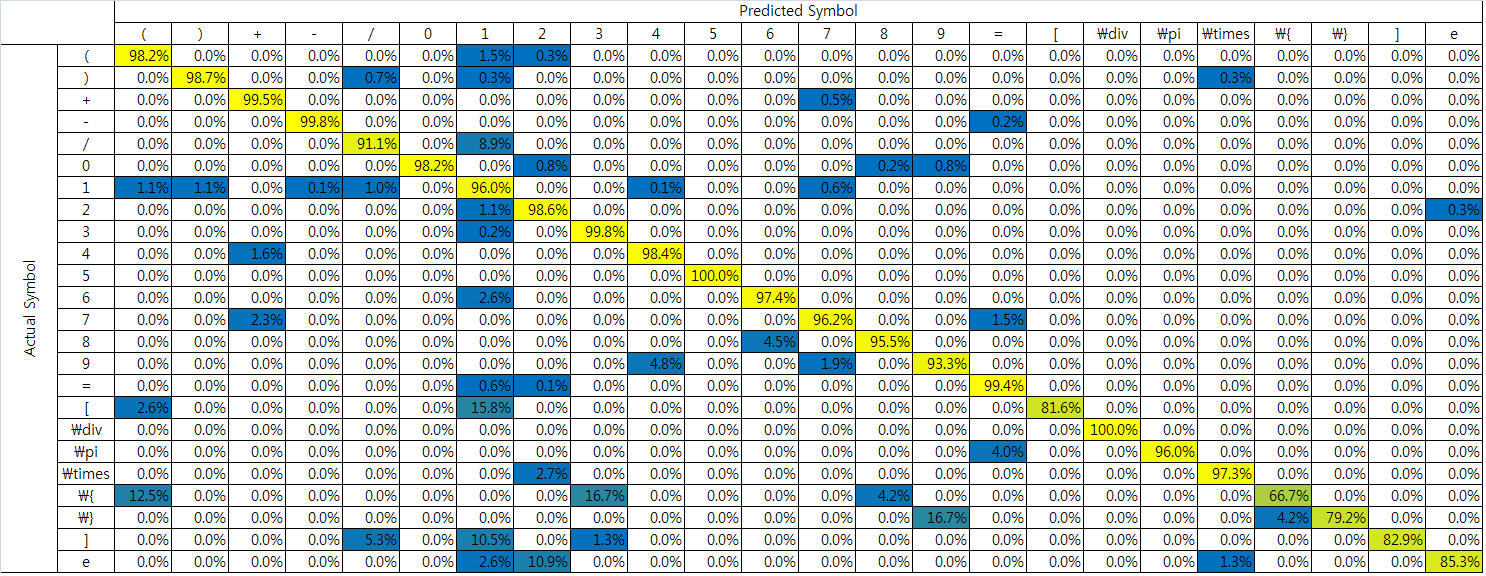
\includegraphics[width=0.95\linewidth]{img/confusion_matrix.png}
\caption{Confusion matrix of trained model.}
\label{fig:confusion_matrix}
\end{figure*}

\subsection{Web Demo}

The web demo is available at \url{http://chanmin.kim/image-expr/}.

\begin{figure}[ht]
\centering
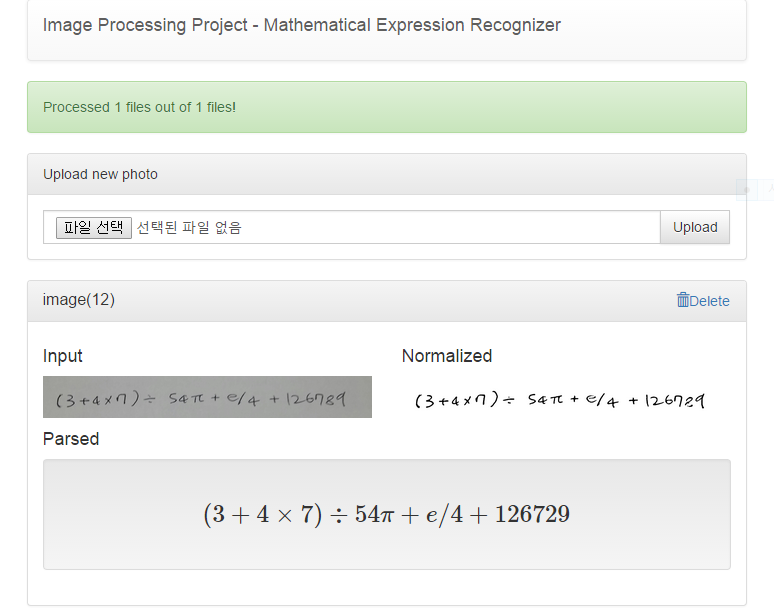
\includegraphics[width=0.9\linewidth]{img/web_demo.png}
\caption{Screenshot of web demo.
Any user can upload drawn or captured images of handwritten expressions.
Then input image, normalized image, and parsed result will appear in a box form.
Unwanted results can be removed.}
\label{fig:thresholding}
\end{figure}

\section{Conclusion}

\subsection{Summary}

% 우리가 한 거 요약이랑, 그런 거

\subsection{Lessons}

% 우리가 이걸로 뭘 배웠는지..

\subsection{Future Work}

% 더 할 수 있을 법한 거?

{\small
\bibliographystyle{ieee}
\bibliography{egbib}
}

\section{Appendices}

\begin{table}[h]
\centering
\begin{tabular}{|l|l|l|l|l|l|l|}
\hline
$($ & $)$ & $+$ & $-$ & $/$ & 0 & 1 \\ \hline
2 & 3 & 4 & 5 & 6 & 7 & 8 \\ \hline
9 & $=$ & $[$ & $\div$ & $\pi$ & $\times$ & $\{$ \\ \hline
$\}$ & $]$ & e & $ $ & $ $ & & \\
\hline
\end{tabular}
\caption{List of symbols recognized by the neural network}
\label{tbl:symbollist}
\end{table}

\end{document}
